\chapter{三维重建的一般方法以及改进}
\label{cha:chap3}
\section{引言}
\label{sec:3.1}
内容内容内容内容内容内容内容内容内容内容内容内容内容内容内容
\section{三维重建的一般步骤}
\label{sec:3.2}
三维重建是指从三维图像中复原三维场景或者物体的过程,整个流程的输入为无序的图片即可,输出可以得到三维重建后的稀疏点云和稠密
点,大致流程如图~\ref{fig:3Dconstr_pipiline_sfm}所示。
\begin{figure}[H] % use float package if you want it here
    \centering
    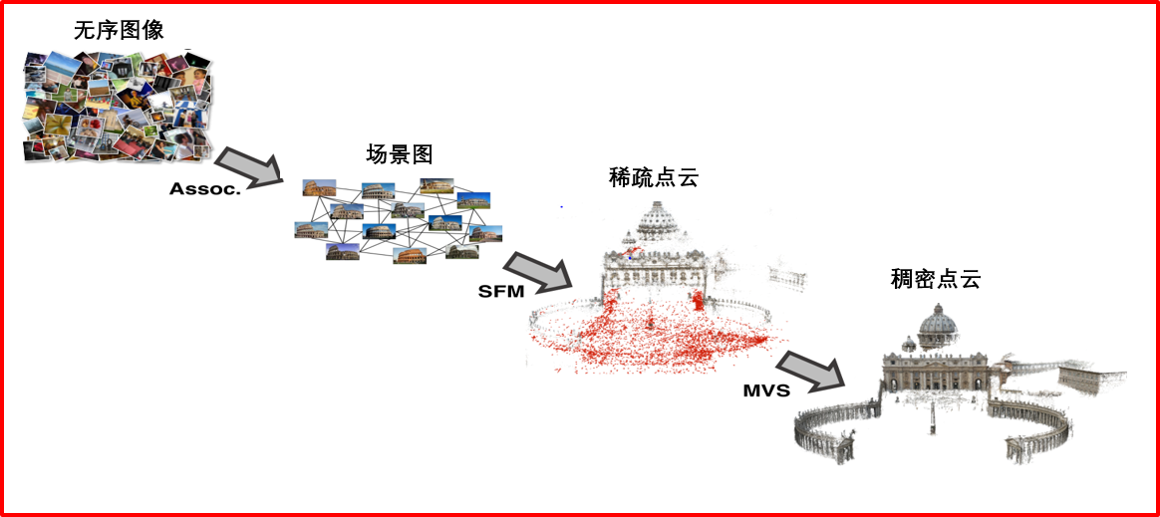
\includegraphics[width=12cm]{3Dconstr_pipiline_sfm.png}
    \caption{三维重建流程图}
    \label{fig:3Dconstr_pipiline_sfm}
    \end{figure}
\subsection{一般方法概述}
\label{sec:3.2.1}
对于以上流程进一步进行细化,整个三维重建的过程可以划分为以下几个主要的步骤:

1.  2D图像采集:多角度拍摄或者从视频中提取到一组图像序列,将图像序列作为整个系统的输入;

2.  特征点提取和匹配:根据拍摄到的图像,提取每张图像之间的特征点,并进行特征点的匹配;

3.  稀疏点云:根据匹配结果估计特征点的深度,提取出稀疏点云,并估计相机的位姿和参数;

4.  稠密点云:根据优化后的相机参数和匹配结果,获得稠密点云;

5.  纹理映射:根据以上点重建物体表面,进行纹理映射。\\
三维重建的一般步骤可以简化为如图~\ref{fig:3Dconstr_pipiline}所示。
\begin{figure}[H] % use float package if you want it here
    \centering
    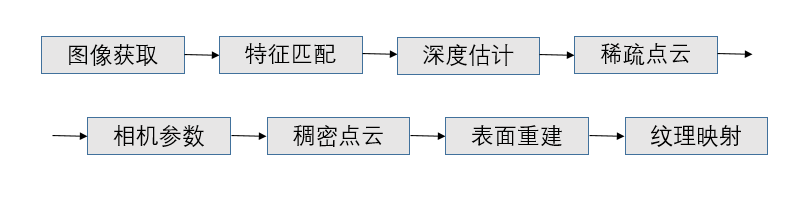
\includegraphics[width=12cm]{3Dconstr_pipiline.png}
    \caption{三维重建一般步骤流程图}
    \label{fig:3Dconstr_pipiline}
    \end{figure}

三维重建主要分为多个步骤,目前很多开源的系统都可以完成其中的部分环节,对于完整的三维重建流程还需要多个系统相互连接实现,
表~\ref{tab:3D_compare}是当前三维重建系统的简要对比。本文在考虑到各个系统流程的完整性和合理性,以及在实际测试过系统之
间的效果差异后,选择Colmap作为作为三维重建的工具。
\begin{table}[h]
    \centering
    \caption{常见三维重建系统对比表}
    \label{tab:3D_compare}
    \begin{tabular}{C{3.6cm}C{2.4cm}C{2.4cm}C{2.4cm}C{2.4cm}}
    \toprule
    \textbf{系统名称} & \textbf{稀疏点云} &\textbf{稠密点云} &  \textbf{重建表面} &\textbf{纹理映射}  \\
    \midrule
    Bundler       &\cellcolor{green}是&\cellcolor{gray}否&\cellcolor{gray}否&\cellcolor{gray}否\\
    CMVS          &\cellcolor{gray}否&\cellcolor{green}是&\cellcolor{gray}否&\cellcolor{gray}否\\
    Colmap        &\cellcolor{green}是&\cellcolor{green}是&\cellcolor{green}是&\cellcolor{gray}否\\
    Meshlab       &\cellcolor{gray}否&\cellcolor{gray}否&\cellcolor{green}是&\cellcolor{green}是\\
    MVE           &\cellcolor{green}是&\cellcolor{green}是&\cellcolor{green}是&\cellcolor{gray}否\\
    MVS-texturing &\cellcolor{green}是&\cellcolor{green}是&\cellcolor{green}是&\cellcolor{gray}否\\
    openMVG       &\cellcolor{green}是&\cellcolor{green}是&否\cellcolor{gray}&\cellcolor{gray}否\\
    openMVS       &\cellcolor{gray}否&\cellcolor{gray}否&\cellcolor{green}是&\cellcolor{green}是\\
    Theia         &\cellcolor{green}是&\cellcolor{gray}否&\cellcolor{gray}否&\cellcolor{gray}否\\
    VisualFSM     &\cellcolor{green}是&\cellcolor{green}是&\cellcolor{gray}否&\cellcolor{gray}否\\
    \bottomrule
    \end{tabular}
  \end{table}
\subsection{维重建详细过程解析}
\label{sec:3.2.2}
\subsubsection{图像获取} 
\label{sec:3.2.2.1}
目前常规的三维重建仅需要输入无序图片,在构图的过程中,可以极大地降低操作的复杂度,并且对于相机的内参和外参也无需
提前提供给整个三维重建的系统,在特征点匹配的过程中,这些参数都可以通过计算得到。对于输入的图像,可以通过随着时间
流单帧拍摄的方式获取或者通过截取视频流的方式得到。在获取图像的过程中,需要注意保证每连续两帧图像之间尽可能保证30$\%$
的重叠区域,相邻两帧之间的旋转角度为30度到45度之间,且物体中的每一个点至少能被三帧图像观测到。
\subsubsection{特征点的检测和匹配} 
\label{sec:3.2.2.1}
目前,在三维重建领域中图像的特征匹配就是以特征点为基础而进行的,所以,如何定义和找出一幅图像中的特征点就非常重要。常见的
特定点检测和匹配主要包括SUFT,SIFT,ORB,Harris角点等,各方法的简要特点如表所示。
\begin{table}[h]
    \centering
    \caption{常见特征检测方法对比表}
    \label{tab:Feature}
    \begin{tabular}{C{4.6cm}L{8.4cm}}
    \toprule
    \textbf{方法名称} & \textbf{特点}  \\
    \midrule
    SUFT&解决特征检测中的尺度不变性问题,具备较高的计算效率\\
    SIFT&以SUFT为基础,基于浮点内核计算特征点,有着更加精确的空间位置和尺度\\
    ORB&满足实时性的速度,但是不具备旋转,尺度不变性且噪声敏感\\
    Harris角点&能够较好的检测角点,进行精确的定位\\
    \bottomrule
    \end{tabular}
  \end{table}

对于本文中的三维重建,选择SIFT作为特征点的检测和匹配方法,针对其计算耗时的问题,本文选择CUDA进行硬件加速,另外还考虑到三维
重建本身是一个离线处理的过程,对算法的实时性没有过高要求。SIFT和其他方法相比较,有以下优点:\\
1. SIFT特征是图像的局部特征,其对旋转、尺度缩放、亮度变化保持不变性,对视角变化、仿射变换、噪声也保持一定程度的稳定性;\\
2. 独特性好,信息量丰富,适用于在海量特征数据库中进行快速、准确的匹配;\\
3. 多量性,即使少数的几个物体也可以产生大量的SIFT特征向量。\\
如图~\ref{fig:3Dconstrmatchresult}所示,分别对两帧图形提取SIFT特征,随后根据特征点进行匹配。
\begin{figure}[H]
    \centering
      \subcaptionbox{第1帧图像提取SIFT特征}{\label{fig::3Dconstr_a}
      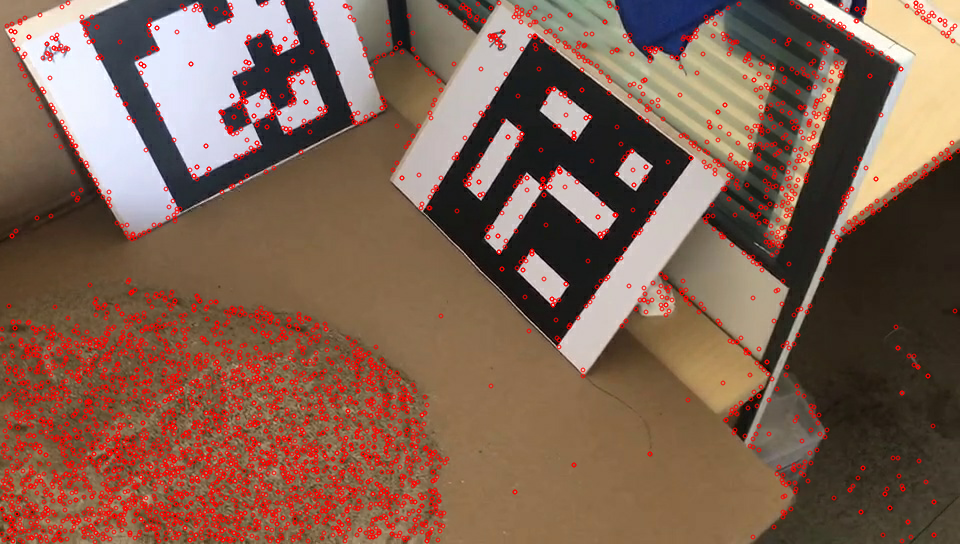
\includegraphics[width=6cm]{3Dconstr_a.png}\hskip2cm}
      \subcaptionbox{第2帧图像提取SIFT特征}{\label{fig:3Dconstr_b}
      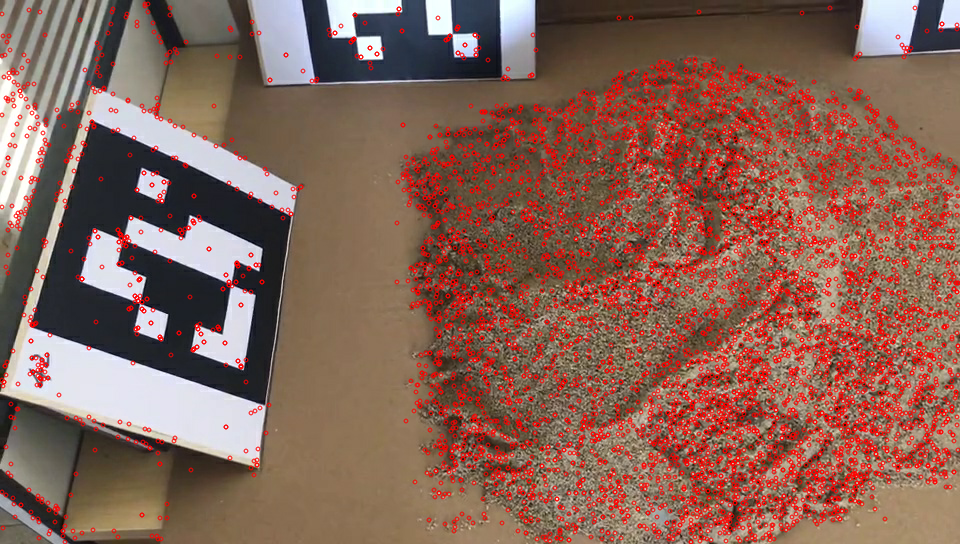
\includegraphics[width=6cm]{3Dconstr_b.png}}
    \vskip0.5cm
      \subcaptionbox{根据特征点进行匹配\label{fig:chap03:3Dconstr_match}}{
      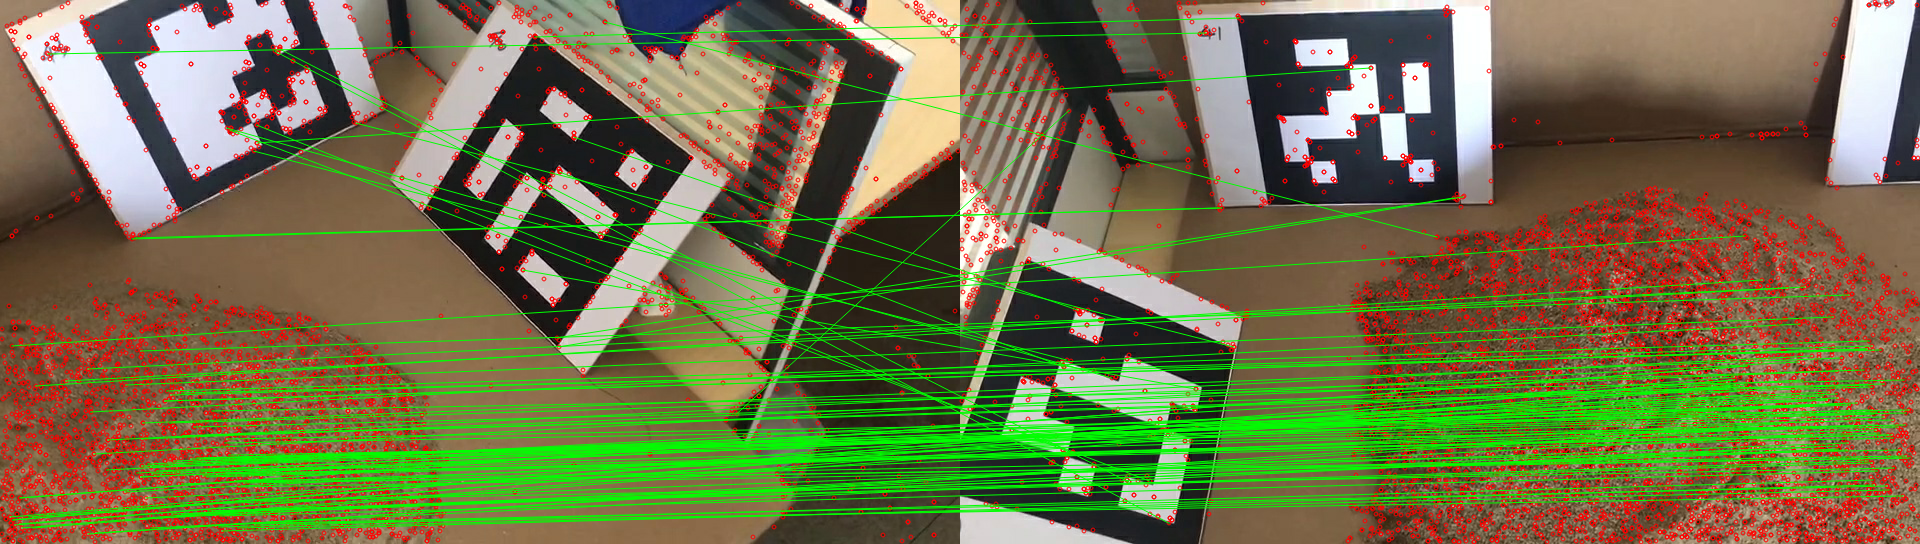
\includegraphics[width=12cm]{3Dconstr_match.png}\hskip2cm}
    \caption{特征提取与匹配结果示意图}\label{fig:3Dconstrmatchresult}
  \end{figure}
由图~\ref{fig:chap03:3Dconstr_match}~所示,两帧之间大多数特征点都可以正确匹配,但依然存在存在部分匹配是错误的,在本文中,
选择了RANSAC(随机抽样一致性)的方式来剔除错误的匹配对,以更加准确的估计相机位姿,RANSAC是指可以从一组包括局外点(错误匹
配)的观测数据中,通过迭代的方式估计数学模式中的参数,通过RANSAC处理后的匹配结果如图~\ref{fig:3Dconstr_matchAfterRansac}
所示,误检的匹配已经被明显的降低。
\begin{figure}[H] % use float package if you want it here
  \centering
  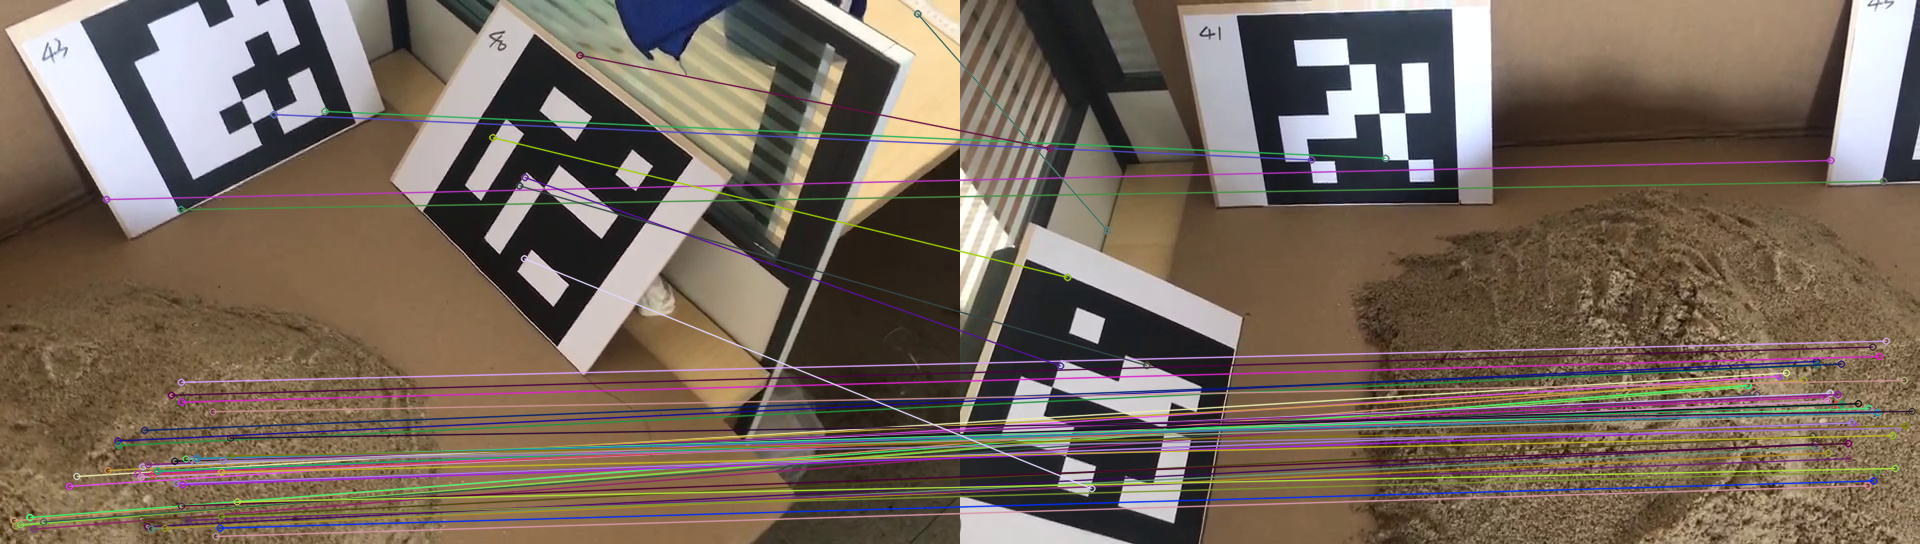
\includegraphics[width=12cm]{3Dconstr_matchAfterRansac.png}
  \caption{RANSAC之后的点云匹配}
  \label{fig:3Dconstr_matchAfterRansac}
  \end{figure}
\subsubsection{获取稀疏点云} 
\label{sec:3.2.2.3}
\subsection{当前三维重建存在的问题}
\label{sec:3.2.3}

